\documentclass{article}
\usepackage{amsmath}
\usepackage{graphicx}
% affil
\usepackage{authblk}

% times new roman, 10pt, 1.5 spacing
\usepackage{times}
\usepackage{setspace}
\setstretch{1.5}
\usepackage{titling}
\setlength{\droptitle}{-4em}

% set margins
\usepackage[top=1.5in, bottom=1.5in, left=1.5in, right=1.5in]{geometry}
% footnotes should be the same size as the main text
\renewcommand{\footnotesize}{\normalsize}



% *** Do not adjust lengths that control margins, column widths, etc. ***
% *** Do not use packages that alter fonts (such as pslatex).         ***

\begin{document}
%
% paper title
% Titles are generally capitalized except for words such as a, an, and, as,
% at, but, by, for, in, nor, of, on, or, the, to and up, which are usually
% not capitalized unless they are the first or last word of the title.
% Linebreaks \\ can be used within to get better formatting as desired.
% Do not put math or special symbols in the title.
\title{Surveying the (loss) landscape: using machine learning to improve household survey accuracy}

% Author: Nikhil Woodruff. Affiliations are:
% University of Durham
% PolicyEngine

\author{Nikhil Woodruff}
\affil{University of Durham}
\affil{PolicyEngine}




%% --------------------------------------------- DO NOT CHANGE ---------------------------------------------

% make the title area
\maketitle

\begin{abstract}
  Microsimulation over survey datasets remains the dominant method for analysing and predicting the impact of government policy. However, the accuracy of these models is often limited by the quality of the survey data. In this paper, I present a novel approach to improving the accuracy of survey data by using machine learning to counter both sampling and measurement error. I evaluate this approach on the UK's Family Resources Survey in combination with other datasets, and benchmark its performance against other state-of-the-art methods including percentile adjustment. I find that the proposed approach is able to improve the accuracy of the survey data as a predictor of more trustworthy statistics from administrative sources (which are not granular enough to be used for microsimulation).
\end{abstract}


% To allow for easy dual compilation without having to reenter the
% abstract/keywords data, the \IEEEtitleabstractindextext text will
% not be used in maketitle, but will appear (i.e., to be "transported")
% here as \IEEEdisplaynontitleabstractindextext when the compsoc 
% or transmag modes are not selected <OR> if conference mode is selected 
% - because all conference papers position the abstract like regular
% papers do.
% Computer Society journal (but not conference!) papers do something unusual
% with the very first section heading (almost always called "Introduction").
% They place it ABOVE the main text! IEEEtran.cls does not automatically do
% this for you, but you can achieve this effect with the provided
% \IEEEraisesectionheading{} command. Note the need to keep any \label that
% is to refer to the section immediately after \section in the above as
% \IEEEraisesectionheading puts \section within a raised box.

%% --------------------------------------------- DO NOT CHANGE ---------------------------------------------




% The very first letter is a 2 line initial drop letter followed
% by the rest of the first word in caps (small caps for compsoc).
% 
% form to use if the first word consists of a single letter:
% \IEEEPARstart{A}{demo} file is ....
% 
% Here we have the typical use of a "T" for an initial drop letter
% and "HIS" in caps to complete the first word.

\section{Introduction}
Governments across the world redistribute trillions of dollars every year through tax and benefit programs. On average, countries collect around a third of their gross domestic product in taxes, and distribute around a third of tax revenues as cash benefits. These programs are ultimately incident on households, either directly or indirectly. Direct taxes and benefits impact households by direct transfers between households and government entities, and indirect taxes or benefits (subsidies) levied on private suppliers manifest themselves in the altered transactions between households and non-government entities. But whether by indirect or direct means, tax-benefit policy represents perhaps the largest single contributor to the state of household finances for billions of people. 

The complex rules defining the behaviour of these programs are set in tax-benefit legislation, and are amended or reformed constantly over decades. While legislators may have different overall goals for tax-benefit policy outcomes, engineering the tax-benefit system to achieve specific intended outcomes requires being able to predict the impact of individual policy reforms on metrics like the budget, the poverty rate, or the distribution of income. Therefore, the accuracy with which researchers can predict the impact of policy reforms is critical.

Researchers largely achieve this through \emph{microsimulation}, a technique which involves simulating the application of tax-benefit program rules on a representative sample of households, using collected data on demographics, household structures, income sources and other features. This technique has been used extensively across both developed and developing countries, and is the dominant method for analysing and predicting the impact of government policy.

Microsimulation models' accuracy is completely dependent on the accuracy of the survey data on which it operates. However, there is evidence to suggest that the surveys which are used in microsimulation models today are at least partially inaccurate, and this inaccuracy may be worse for specific use-cases.

Machine learning has emerged as a powerful tool for data transformation tasks, including synthetic data generation, across many social science subfields. However, the field of tax-benefit microsimulation has been largely untouched by it in the decades that it has been the standard. This paper aims to address this gap by proposing a novel approach to improving the accuracy of survey data by using machine learning to counter both sampling error (by gradient descent-based reweighting) and measurement error (by random forest model-based synthetic data generation). I evaluate this approach on the UK's Family Resources Survey in combination with other datasets, and benchmark its performance against other state-of-the-art methods including percentile adjustment. I find that the proposed approach is able to substantially improve the accuracy of the survey data as a predictor of more trustworthy statistics from administrative sources (which are not granular enough to be used for microsimulation).

\subsection{Microsimulation}

\emph{Tax-benefit policy microsimulation} has emerged over recent decades as the dominant method for analysing and predicting the impact of government policy. This technique involves simulating the application of tax-benefit program rules on a representative sample of households, using collected data on demographics, household structures, income sources and other features.

In the United Kingdom, the most comprehensive household survey is the Family Resources Survey (FRS). This survey is collected annually by the Department for Work and Pensions, and includes approximately 20,000 households in a given year. Estimates for population-level features (such as the median income) can be derived using individual weights for household records which indicate how many UK households each respondent is representative of. However, despite a weight generation procedure that aims to ensure accurate representation of the UK household sector, prior research has found that the survey does not accurately predict household statistics well at the very-low or very-high ends of the income distribution: benefit aggregates derived from the FRS are around 20\% lower than the in administrative benefit databases, and top income percentiles are lower than than in HMRC's administrative tax database.

There are two ways that a survey can diverge from the reality of the target population: sampling error and measurement error. In the microdata, measurement error arises where the values of individual observations are incorrect (not necessarily through deliberate deceit from survey respondents- question design and integrity checks can influence the accuracy of responses). Sampling error arises where the sample of respondents is not representative of the target population, primarily manifesting as an incorrect weighting of the household records. Both of these sources of error interact with each other: correcting for a missing household subsector can either be achieved by increasing the weight of an existing record or by transforming the values of another record.

Inaccuracy in survey data has real-world impacts: by negatively affecting the accuracy of tax-benefit policy microsimulation, survey inaccuracy can distort the conclusions of policy evaluations, leading to suboptimal government policy design. Where surveys consistently under-represent particular subsectors of the household sector, this can lead to a systematic bias in the policy evaluation process and distort public understanding of the impact of government policy. Many existing methods for mitigating these types of inaccuracy make heavy use of arbitrary assumptions about the distribution of survey data variables. For example, in correcting for the under-representation of high incomes, a common approach is to match the top income percentiles of a household survey to percentiles from administrative tax datasets. This can achieve exact parity between the two datasets on this very specific target metric, but this introduces significant risk of overfitting: of all the questions that we could ask of the survey data, income percentiles are a small fraction, and other targets could plausibly be thrown off by this adjustment.

\subsection{Objectives}

This project aims to evaluate a novel use of a combination of machine learning-based techniques to correct for household survey inaccuracy from both sampling and measurement error, and to compare its performance against other state-of-the-art methods. This approach involves using random forest model inference to synthesise new records, and then using gradient descent to minimise a constructed loss function that measures the deviation of the household survey from a large set of official statistics.

To assess the value-add of the resulting pipeline, I will compare the performance of its application on the UK's Family Resources Survey, against several different state-of-the-art alternatives:

\begin{itemize}
  \item The original, un-modified FRS
  \item The FRS modified with percentile adjustment (a common method for correcting for under-representation of high incomes)
\end{itemize}

Since the pipeline in this project is a composite of several different (optional) stages, I will also compare different configurations (for example, removing the synthetic data extension element) of the pipeline in order to estimate the value of each individual stage.

If the pipeline is found to be effective, it could be used to improve the accuracy of tax-benefit microsimulation models, and therefore improve the accuracy of policy evaluations. This could lead to more accurate policy design, and more accurate public understanding of the impact of government policy.

\section{Related Work}
This section presents a survey of existing work on the problems that this project addresses. It should be between 2 to 3 pages in length. The rest of this section shows the formats of subsections as well as some general formatting information for tables, figures, references and equations.

Over the last few decades, there has been extensive research into the accuracy of household surveys for estimating socioeconomic and policy-related indicators, as well as methods of improving survey accuracy. Most of these studies have focussed on one particular mechanism by which surveys introduce inaccuracy (for example, by omitting top incomes or under-sampling low incomes), and examine a method of improving surveys which tackles this particular flaw. This literature survey aims to provide a comprehensive overview of the state of the art in improving survey accuracy, while also examining how and if these individual advancements complement each other.

\subsection{Current approaches in economic surveys}

It is well known that household surveys produce inconsistent results to other data sources, such as administrative databases. Given the nature of how surveys are conducted (households must first consent to an interview, and secondarily must answer truthfully to questions asked), this inaccuracy can be introduced either by sampling error or measurement error (likely both, to some extent). Over the last few decades, household surveys have become the dominant tool in measuring and projecting economic impacts of policy changes, and as such, there has been a great deal of research into improving survey accuracy.

\subsubsection{Under-coverage of high incomes}

The Department for Work and Pensions is required by law to report on poverty and inequality metrics every year, and in meeting this requirement, it publishes a household-level dataset of disposable incomes, termed the Households Below Average Income (HBAI) dataset.\cite{hbai} Since 1992, it has applied an adjustment to the disposable incomes of a subset of the dataset in order to make the coverage of top incomes more comparable with that of HMRC's Survey of Personal Incomes (SPI) dataset - this adjustment termed the `SPI adjustment'. In \cite{ifs_survey_under_coverage}, the authors examine the methodology of this adjustment, as well as its performance against its original goals.

The authors document\footnote{Previously, the DWP had not published its research underlying the methodology of the SPI adjustment} the steps of the SPI adjustment, which involve first identifying a set of `rich' households. The definition of rich applies a condition that a household's income must be above a certain threshold, where separate thresholds are used for pensioner and non-pensioner households. The target used to set thresholds is generally to ensure that around 0.5\% of records are altered, varying by year. The HBAI `rich' households are then modified by replacing gross incomes (an income measure which the SPI also contains) with the average values for records in the same group in the SPI. Finally, the survey weights are recalculated: in the original survey, weights are solved by matching administrative statistics on population sizes; under the SPI adjustment, population sizes of the `rich' groups are included in the set of statistical targets to hit. The authors find that the SPI adjustment has been successful in improving the coverage of top incomes in the HBAI dataset, but raise a number of issues:

\paragraph{Income decomposition} The SPI adjustment is applied to a singular income variable, but the FRS contains a number of components. Modifying gross income, but not modifying employment income, savings income, etc. breaks the link between these variables, which prevents researchers from conducting decomposition analyses.
\paragraph{Stratification} There is no obvious justification for separate thresholds for pensioners and non-pensioners (and further, between households in Great Britain and Northern Ireland). The authors suggest these stratification choices were made in order to minimise methodological changes over time, for example as the survey expanded to Northern Ireland.
\paragraph{SPI lag} The Survey of Personal Incomes is not routinely available at the same time as the Family Resources Survey (from which the HBAI microdata is derived). Therefore the SPI adjustment is applied to the HBAI dataset using a lagged SPI dataset, which may introduce additional inaccuracy.

\subsubsection{Adjustments using administrative tax data}

For the 2019 edition of the Households Below Average Income series, the ONS published details of the methodology used to tune the dataset with the SPI in \cite{ons_spi_version_2}. They respond to some of the concerns raised by \cite{ifs_survey_under_coverage}:

\paragraph{Pensioner stratification} The authors show that high-income pensioners and non-pensioners are both under-represented in their respective populations but comparing the ratios of incomes at different quantiles, finding that a common threshold for both groups would fail to ensure that pensioners (who have lower income, on average) are sufficiently affected by the SPI adjustment.

\paragraph{Choice of income threshold} The authors discuss possible justifications for a particular income threshold, mostly based on the quantile at which divergence between the FRS and SPI `became an issue'. However, the choice to use a binary variable (rather than, for example, phasing in an SPI adjustment) here is arbitrary, and the authors do not address the reasons why this choice was made.

\paragraph{SPI lag} The authors acknowledge the issue of using SPI projections, rather than actual outturn data, and examine the size of this effect. They find that revising recent survey releases with the actual SPI data later released changed the Gini coefficient of income inequality estimates by around 0.2 percentage points. This is considered to be small and therefore recommend against the need for the ONS to re-publish statistics when current SPI data becomes available.

\subsubsection{Capital income imputation}

The issue of income decomposition remained largely untackled until \cite{frs_capital_income}, in which the authors attempt to improve the reporting of a specific component of gross income which is more severely under-reported in the FRS than others: capital income. They first establish that income under-reporting is mostly due to this particular category by comparing individual income sources between the FRS and SPI, finding that the aggregates of non-capital income are around 100\% of the totals for the SPI, while capital income is only around 40\% as represented.

The authors present a novel observation about the instances where capital income is under-reported: the capital share of income in individuals is far less represented in the FRS than in the SPI (specifically, the number of individuals with a `high capital share'), rather than simply a lack of high-capital-income individuals. They introduce a new method to correct for this under-capture: adjust the weights of high-capital-share individuals in order to match the totals in SPI data.

The authors find that the new method is largely successful at correcting for under-capture of capital income, and increases the Gini coefficient of FRS data by between 2 and 5 percentage points (applying the methodology to historical FRS data releases). However, they do not measure the changes to how well the FRS ranks against other aspects of the SPI.

\subsubsection{Under-coverage of very low incomes}

In \cite{brewer_low_income_coverage}, the authors examine the other end of the income spectrum, finding that very low-income households tend to spend much more than moderately low-income households in the Living Cost and Food Survey (a household survey with similar administration to the FRS). The authors report a variety of evidence that income at the low end is misreported in the survey:

\paragraph{Missing benefit spending} By comparing total reported receipt of benefits by recipients with aggregate spending figures published by the DWP and HMRC, the authors find that the FRS and LCFS consistently under-report benefit income by around 5\%, and that this figure has become worse over the last decade, rising from 2.5\% in 2000.

\paragraph{Sub-minimum wage reporting} In the LCFS, individuals report both hours worked and annual earnings, enabling researchers to calculate the implied hourly wage. For 10.5\% of individuals in 2009, this was below the legal minimum wage. Although this does not guarantee a breach of employment law,\footnote{Employers can count some in-kind benefits as payment towards the minimum wage, and there are other legal exceptions.} the proportion is substantial and implies that either earnings are under-reported or hours worked are over-reported. The authors use a model of consumption smoothing to determine whether the overly high spending (compared to income) for low-income households can be explained by lifetime consumption smoothing, but find that this is not the case.

\subsubsection{Linking data directly to administrative data}

All of the previously covered research into survey inaccuracy has identified a common question: how much of the survey error is due to non-response bias, and how much is due to measurement error? In \cite{dwp_110}, the authors attempt to quantify the measurement error of the FRS by linking individual households with data from the DWP's administrative records, using non-public identifiers. The process of linking is not perfect: respondents are asked for permission to link their survey data with administrative data, and some (around 30\%) refuse. However, for each benefit, the authors were able to find the percentage of reporting adults for whom a link to an administrative data record could be identified, the percentage of reporting adults recipients for whom no link could be found, and the percentage of adults represented only by administrative data. 

The authors find that these splits vary significantly by benefit: recipient data on the State Pension (SP) is highly accurate in the FRS (96\% of SP reported recipients were represented by the FRS, 1\% were only on the FRS and not on administrative datasets, and 3\% were only on administrative datasets). At the same time, around 62\% of adults on the FRS who reported receiving Severe Disablement Allowance could not be identified in administrative data. There are multiple possible reasons for this, and they vary by benefit: the recipient population is often confused or mistaken when answering questions about their benefits, and this is more acute for age- or disability-related benefits. This appears to provide additional evidence that measurement error is significant, at least at the low-income subset of the surveys.

\subsubsection{Linear programming}

Linear programming, a mathematical technique for solving linearly constrained optimisation problems, is commonly used to determine survey weight values, where the criteria are defined maximum deviations from top-level demographic statistics. In \cite{frs_weighting_review}, linear programming methods are used to determine the optimal weights for the Family Resources Survey, according to limits on how far apart the FRS aggregates can be from national and regional population estimates. In both of \cite{tpc_microsim_docs} and \cite{taxdata_github}, tax models apply a linear programming algorithm to solve for weight adjustments satisfying a combination of tax statistic deviation constraints, and weight adjustment magnitude limits.

\subsection{Applicable machine learning techniques}

There are several reasons why machine learning techniques are well-suited to the task of survey imputation. The most fundamental justification is in its context-agnostic nature: machine learning approaches do not require assumptions specific to the field they are applied in, unlike the current approaches to survey accuracy improvement (for example, the percentile adjustment methodology in \cite{ons_spi_version_2}, which explicitly partitions households into `rich' and `non-rich' using arguably arbitrary definitions). In other domains, for example image classificaion, a move away from prescriptive methods towards loss function minimisation has seen substantially improved accuracy and robustness.\cite{image_classification_survey}

\subsubsection{Gradient descent}

Gradient descent is a technique for finding parameters which minimise a loss function, by iteratively updating the parameters in the direction of the steepest negative gradient.\cite{gradient_descent} This is a highly common technique in machine learning, and is used in a variety of contexts, most notably as the foundation for training artificial neural networks. It relies on no domain-specific assumptions other than those present in the definition of the loss function, enabling it to be applied to a wide range of problems.

Several variations of gradient descent have emerged over the years which achieve more efficient training procedures: stochastic gradient descent steps in the direction of an \emph{estimate} of the gradient using individual training examples, rather than loading the full dataset.\cite{sgd} Mini-batch gradient descent represents a compromise between batch (full-dataset) and stochastic gradient descent, by iterating parameters using fixed-size subsets of the training data.\cite{mini_batch}

As well as gradient calculation methods, optimisation algorithms have revealed significant accuracy and efficiency improvements by defining behaviours for hyper-parameters such as the learning rate (the velocity at which parameters follow the gradient). These include Adam,\cite{adam} AdaGrad,\cite{adagrad} and RMSProp.

Gradient descent could feasibly be applied to survey accuracy problems, since it requires only a loss function that is differentiable with respect to the parameters being optimised. In the context of survey accuracy, a loss function could be defined as the squared errors of individual aggregate statistics between official sources, and a survey, which would be continuously differentiable over the weights of individual household records.

\subsubsection{Random forest models}

Random forest models are a type of ensemble learning technique, which combine the predictions of multiple decision trees to produce a more accurate prediction than any individual tree.\cite{random_forests} The decision trees are trained on a subset of the training data, and the predictions of each tree are combined using a voting system. Although its introduction is far less recent than more modern innovations in the field of neural networks (for example, artificial neural network variants\cite{anns} or transformers\cite{transformers}), random forest models have shown consistently high accuracy across a wide range of domains, remaining competitive with the most recent techniques.

This type of model has been applied (to a limited extent) in the context of policy analysis, and have shown superior performance in prediction tasks to logit and other model types.\cite{ecb}

There are several reasons why random forest models might outperform neural networks in predicting survey microdata values from other attributes (for example, predicting employment income from demographic variables), but the most natural reason is that tax-benefit law, which heavily influences financial decisions, is more similar in structure to a random forest than a neural network. For example, in \cite{cg_bunching} the authors found that capital gains variables are `unnaturally' distributed in order to respond to incentives set by particular tax law parameters.

\section{Methodology}



\subsection{Loss}

\subsubsection{Concept}

The loss function is the function that is minimised by the optimisation algorithm. In the context of survey imputation, the loss function is the difference between the survey aggregate statistics and the official aggregate statistics. The loss function is defined as:

\begin{equation}
  L(S) = \sum_{c \in C} L_c(S)
\end{equation}

where $L_c(S)$ is the loss function for a particular aggregate statistic $c$, $C$ is the set of all aggregate statistics and $S$ represents a given household survey (a collection of relational databases). The loss function for a particular aggregate statistic $c$ is defined as:

\begin{equation}
  L_c(S) = w * (\frac{\sum_i^{N} X_i \cdot max(W_i, 0)}{y} - 1) ^ 2
\end{equation}

where $X_i$ is the value (of a particular variable) of the $i$th household record, $W_i$ is the weight of the $i$th household record, $y$ is the official aggregate statistic for $c$, and $w$ is a weighting factor for the loss function. The weighting factor $w$ is used to prioritise certain aggregate statistics over others (for example, budgetary impact size is used to comparatively weight different financial aggregate statistics). The loss function is also hierarchical, in that each loss category contains a weighted sum of other (normalised) loss functions. For example, the loss function for demographic performance might contain subcategories measuring performance over household population targets as well as individual population targets.

Note that the weight $W_i$ is constrained to be non-negative, since negative weights do not have a meaningful interpretation in the context of survey imputation.

\subsubsection{Normalisation} There remains an issue in how to constrain the relative sizes of different loss values. For example, we might have many more detailed statistics over which we can evaluate the survey in its representation of Income Tax (revenues by income band, taxpayer counts) than we do for Child Benefit (only aggregate revenue and total claimants). Naively summing the relative error comparisons for each category would give Income Tax targeting a much higher weight in the optimisation process purely because of our access to statistics (which is no indication of a program's importance). Simply dividing by the number of comparisons would be inaccurate too, given some of those comparisons might be more important than others. Therefore instead, a more neutral assumption is to normalise each loss category by dividing by its initial value:

\begin{equation}
  L(S) = \frac{\sum_{c \in C} L_c(S)}{L(S_0)}
\end{equation}

The question of how to determine the weighting factor for each loss function is also arbitrary, but the most neutral assertion could be to use the aggregate financial size of a program, or the size of the population concerned. For example, if we have one loss category measuring how well the survey reproduces Income Tax statistics and another measuring Child Benefit, we could reasonably consider that the Income Tax loss category is approximately twenty times more important than the Child Benefit loss category\footnote{Income Tax revenue in 2022 was around £200 billion, while Child Benefit outlays were around £10 billion.}.

This paper benchmarks the performance of the survey accuracy improvement pipeline by focussing on UK survey data, which requires an implementation of the loss function for the UK context. The UK loss function is defined using the following categories:

\begin{enumerate}
  \item Demographics
  \begin{enumerate}
    \item Households
    \begin{enumerate}
      \item Region-Council Tax Band intersections*
      \item Region-tenure type intersections*
    \end{enumerate}
    \item Populations
    \begin{enumerate}
      \item Age-sex-region intersections*
    \end{enumerate}
  \end{enumerate}
  \item Programs
  \begin{enumerate}
    \item Universal Credit$^\dagger$
    \item Child Benefit$^\dagger$
    \item Child Tax Credit$^\dagger$
    \item Working Tax Credit$^\dagger$
    \item Pension Credit$^\dagger$
    \item Income Support$^\dagger$
    \item State Pension$^\dagger$
    \item Housing Benefit$^\dagger$
    \item Income-based ESA$^\dagger$
    \item Income-based JSA$^\dagger$
    \item Council Tax$^\dagger$
    \item National Insurance$^\dagger$
    \item Employment income$^\dagger$
    \item Self-employment profit$^\dagger$
    \item Private pension income$^\dagger$
    \item Savings interest income$^\dagger$
    \item Property income$^\dagger$
    \item Dividend income$^\dagger$
    \item Income Tax$^\dagger$
    \begin{enumerate}
      \item Taxpayers by UK nation
      \item Tax liability by 10 income bands
    \end{enumerate}
  \end{enumerate}
\end{enumerate}

Loss categories marked with * contain statistics that are also used to determine the original FRS survey weights. Categories marked with $^\dagger$ include aggregate financial size and non-zero counts by UK nation, weighted by the aggregate financial size of the program. For example, the program loss categories is approximately defined by:
\begin{equation}
  \begin{split}
  L_{Programs}(S) &= 45 \times 10 ^ 9 L_{Universal Credit} (S)\\& + 11 \times 10 ^ 9 L_{Child Benefit} (S)\\& + \dots\\& + 200 \times 10 ^ 9 L_{Income Tax} (S)
  \end{split}
\end{equation}

This is necessary, since loss categories in themselves are normalised and expressed as a percentage of the first loss value.

\subsection{Gradient descent}

A given survey $S$ is itself a set of variables $X_{i,j}$ (where $i$ is the household record and $j$ is the variable), as well as household weights $W_i$.\footnote{Although most household surveys also include personal and family weights, only the household weights are optimised in this project.} We can therefore split up the loss function to be a function of the variables and weights separately (and implementing this split is achievable in the underlying algorithm code) as $L(S) = L(X, W)$. Our loss minimisation task therefore becomes finding the solution to Equation \ref{eq:gradient_descent}.

\begin{equation}
  % Solve for the derivative being zero.
  \frac{\partial L(X, W)}{\partial W} = 0
  \label{eq:gradient_descent}
\end{equation}

The loss function for a specific household survey will be a large set of composite functions incorporating hundreds of individual targets, but the gradient function can be analytically calculated using automatic differentation packages such as PyTorch.\cite{pytorch} Under the gradient descent algorithm\cite{anns}, the weights are iteratively updated in the direction of the steepest negative gradient, until the loss function is minimised.

\subsection{Imputation}

There are several reasons why reweighting alone will likely not be sufficient to eliminate certain types of error in the survey. For example, suppose that one of the income tax targets involves the revenue from certain high-income tax filers. A survey which does not include any instances of these filers will categorically be unable to make any progress towards this target. This case does occur frequently in practice: the highest taxable income in the Family Resources Survey (2020-21) is less than £1m, but HMRC reports aggregate tax revenues from filers with incomes over this level in the order of £1bn.

This problem manifests as a global minimum floor in the loss landscape over the space of the original survey weights, below which no optimisation improvement is capable of reaching. To circumnavigate this barrier, we must add new records and weights to the parameters optimised by the gradient descent algorithm.

Synthesing new records to add to the existing survey brings risks: we could decrease the accuracy of the survey by adding new records which are unrealistic. This is not a concern: it can be avoided entirely by adding new records with weight values set to zero, since this does not actually change the result of anything produced with the survey, and instead just provides the optimisation algorithm with more parameters to change. However, while synthesising implausible records cannot harm the survey, it is likely that the more plausible the new record, the better it can aid the optimisation routine.

There are a variety of machine learning-based methods for synthesising new data points from a learned distribution. In \cite{ghenis_quantile_regression}, Ghenis benchmarked several of these methods against each other and found that a random forest model-based approach minimised \emph{quantile loss}, an indicator of how well the distribution of generated values aligns with the prior distribution, the most. Preserving heterogeneity in distributions is important here: microsimulation modelling's core strength comes from its ability to simulate independent outcomes across a highly diverse sample of the population.

This leaves the question of from which distribution we should synthesise new records. Clearly, this should not be the Family Resources Survey given this would be self-defeating. A data source more likely to produce success would be HMRC's Survey of Personal Incomes: a 1\% (anonymised to meet disclosure rules) sample from HMRC's administrative tax records. The SPI does not suffer the same under-counting of incomes (in fact, its aggregates are the basis by which we know the FRS is inaccurate), and the inability of individuals to refuse to participate in the survey means that it is likely to be more representative of the population than the FRS. Therefore, since SPI records are able to reproduce SPI aggregates, SPI-like records sampled from the SPI in FRS format should be able to move FRS aggregates in the direction of SPI aggregates when given enough weight.

The structural form of the model to use is distinct from how it mechanically integrates with the rest of the survey enhancement pipeline. The exact method we use is set out in the following steps:

\begin{enumerate}
  \item Identify common variables between the SPI and the FRS.
  \item Partition these into two sets: the predictor set and the imputation set.
  \item Train a random forest model to predict imputation set variables given the predictor set variables.
  \item Duplicate each household record once, assigning zero weight to the copy.
  \item For each household record in the FRS, use the random forest model to predict the imputation set variables.
  \item Override the imputation set variables in the copied household record with the predicted values.
\end{enumerate}

At the end of this process, the new FRS dataset is identical to the original dataset because the new additions are zero-weighted. However, the optimiser now has a far expanded parameter space to work with, and can therefore (potentially) make more progress towards the target.

\subsubsection{Distribution adjustment}

However, even if we can accurately capture the relationship between variables in a more accurate dataset, this doesn't guarantee that applying the model to the FRS will produce the same record distributions as in the SPI, because the SPI and FRS have different sampling frames: imputing income variables might correct for the FRS undercounting high incomes \emph{among people who would have high incomes if HMRC were asking}, but the FRS also will have less of these people than would exist in the SPI (due to sampling bias).

Another pitfall of the imputation method is that it might not produce the most efficiently loss-potential-reducing records (from the perspective of the space they take up), or might even fail to produce the specific records that exist in reality but not in either survey. For example, many of the individuals with the highest incomes will not appear even in the SPI. How can we ensure these records are created? One naive approach would be to simply craft them by hand, but this is both not scalable, and also might introduce inaccuracy if the hand-made records have some unseen internal contradiction that would mean they cannot exist in real life. Instead, we can preserve the strength of our random forest models at capturing relationships between variables, and just adjust the distribution they predict.

Random forest regressors use the average of the results of a tree set as their outputs. The outputs from each tree incorporate all the learned information about the output variables conditional on the input variables, making it the optimal interception point to modify the model outputs without sacrificing the model's learned relationships. We can from here change the output from an average over all trees to a given percentile of the tree results. Since heterogeneity is still important, this percentile (per household observation) can be sampled randomly from a distribution (evenly and centered at 50\% by default). Parametrising this distribution as a Beta distribution allows us to control its skew by a set parameter.\footnote{The Beta distribution is parametrised by two parameters, but it is trivial to express this as one.} Adjusting this skew parameter now enables us to adjust the distribution of predicted values upwards or downwards as needed.

\subsubsection{Multivariate prediction}

Multivariate prediction might need to make use of separate distribution parameters for individual variables (e.g. if dividend income is more likely to be under-represented by sampling bias than employment income). To allow for this while still retaining consistency between predicted variables, we can train individual variable predictive models on the sequential predictor variables. For example, if we are to predict employment income and dividend income from age, we would train one model predicting employment income given age, and another predicting dividend income given age and (previously predicted) employment income. This is a straightforward extension of the univariate case, and can be implemented in the same way.

\subsection{Data ageing}

The existence of \emph{data lag}, in which a household survey data belongs to a previous year (often 2-3 years before the current), presents a problem for its accuracy in many household surveys and this project. If we have a survey with taxes and benefits from 2019, are are optimising weights to fit statistics from 2022, the optimiser might struggle to perform well (because we are essentially asking it to sample a realistic set of 2022-like households as best it can from a set of 2019-like households). This problem is made worse the more tax and benefit policy changes between the survey year and the target year (and there have been substantial changes in tax-benefit policy, in particular over the pandemic years).

To fix this, we can use a microsimulation tax-benefit model to correct policy-influenced data in the survey. Such a model is a predictor of a set of tax and benefit-related variables (e.g. Income Tax, Universal Credit, etc.) from a set of input variables (e.g. employment incomes, household structure, etc.). Therefore, we can apply this process to each household in the survey data, and correct the relevant variables with those simulated by the microsimulation model, according to 2022 policy.

There are multiple microsimulation models capable of this for UK policy, though only one is both publicly available and open-source: PolicyEngine-UK\cite{policyengine_uk}, which is therefore used in this project.

\subsection{Data pooling}

The FRS has a sample size of around 20,000 households. This can reasonably expected to be enough for the optimiser to be able to obtain good performance, but there are specific reasons why it might not. The largest likely problem is Universal Credit (UC), the UK's central means-tested benefit. Universal Credit is currently being phased-in across the UK, as a replacement for six previous `legacy' benefits, the bulk of which happened between 2019 and 2022. This means that the 2019-20 FRS has a significantly lower share of households claiming Universal Credit (but instead claiming legacy benefits) than would be realistic for 2022. The problem becomes clear if we consider the case of optimising weights to a year in which Universal Credit is fully rolled-out: all the 2019 households with legacy benefits would be essentially worthless, because they would have to be zero-rated in order to not produce erroneous aggregates.

This issue can't fully be solved by data ageing: since there is still some mix of Universal Credit and legacy benefits, the microsimulation model must decide which to simulate based on which benefit the households report already receiving. We could in theory override the households' UC-legacy status to match the rollout percentage, but this might introduce inaccuracy in the household records.

Instead, a cleaner solution is simply to pool multiple years of the survey (before data ageing), in order to increase robustness against this issue of small sample sizes. For this project, we can combine the 2018-19, 2019-20 and 2020-21\footnote{This data release exists, but we do not use it in the default case due to concerns about reliability given lower participation and telephone interviewing (due to the pandemic). Using it here, only given weight at the whim of the optimiser avoids this issue.} datasets (with only the 2019-20 dataset given its initial weights and the others zero).

\subsection{Overall method}

The final, combined pipeline is as follows:

\begin{enumerate}
  \item Combine the three consecutive FRS years into a single dataset.
  \item Duplicate the dataset.
  \item Train the random forest models on income data from the SPI.
  \item Solve for the distribution parameters for each variable s.t. SPI aggregates are reproduced in the model's weighted FRS predictions.
  \item Impute on the FRS and replace-impute income variables from the SPI in the second half of households.\footnote{At this point in the process, the resultant dataset contains six version of the FRS, and only the second (the 2019-20 FRS) has nonzero weights.}
  \item Step through the gradient descent algorithm to minimise survey loss w.r.t. the household weights of the resultant dataset.
  \item Measure the relative change in survey loss from the original dataset.
\end{enumerate}

In order to measure the success of the process, we can record the loss value from the 2019-20 FRS, and compare against the loss for the optimised-pooled-imputed FRS, as well as any alternate versions of the FRS for comparison. 

\subsection{Implementation details}

The implementation\footnote{Full model code, documentation and results is available at https://github.com/nikhilwoodruff/survey-enhance.} for this pipeline is in Python, using the Pytorch library for the gradient descent routine and the Scikit-learn library for the synthetic data generation. For the gradient descent optimisation, I trained the weights for 256 epochs with a learning rate of 1 (given the weights are un-normalised by design, and in the order of 1,000). Random forest models were trained with 100 trees and a maximum depth of 10. For training, I used the default Google Colab environment for reproducibility.

\section{Results}

The implementation of the survey enhancement routine is publicly available as a Python package (\texttt{survey-enhance}), and with public documentation.\footnote{Documentation available at https://nikhilwoodruff.github.io/survey-enhance}. The package is available on PyPI and can be installed with \texttt{pip install survey-enhance}. This package contains the main survey enhancement routines for reweighting and synthetic data generation, and includes an example application in the UK context.

\subsection{Comparison against other methods}

To validate the performance of the pipeline (and its components), we need a unified metric for survey accuracy (a mapping of household surveys to $R$-space). For this, we can use the original loss definition described in the method (for overfitting concerns, see the experiments in REF that validate against this). We can then compare the loss values for each of the following datasets:

\begin{itemize}
  \item Original 2019-20 FRS: the original dataset, with no changes.
  \item Percentile-matched (all) FRS: the FRS with percentiles for all major income sources matched to the SPI.
  \item Percentile-matched (dividends only) FRS: the FRS with percentiles for dividend income only matched to the SPI.
  \item Percentile-matched (pensioner split) 2019-20 FRS: the FRS with percentiles for all major income sources matched to the SPI, but with separate distributions for pensioners and non-pensioners.
  \item Gradient descent-based reweighting: the FRS with weights optimised using the gradient descent algorithm.
  \item Imputed and reweighted FRS: the FRS with zero-weighted, FRS-structured, SPI-sampled synthetic records added, and weights optimised using the gradient descent algorithm.
\end{itemize}

The same hyperparameters for all machine-learning-based models were used between training runs in these comparisons. Table \ref{tab:loss_reduction} shows the change in total normalised survey loss under each survey improvement method.

\begin{table}[!ht]
  \caption{Loss reductions under different survey improvement methods}
  \label{tab:loss_reduction}
  \centering
  \begin{tabular}{cc}
    \hline\hline
    Adjustment & Loss change \\
    \hline
    Percentile matching (all) &      +3.92\% \\
    Percentile matching (pensioner split) &      +0.90\% \\
    None &       0.00\% \\
    Percentile matching (dividends only) &      -0.13\% \\
    Gradient descent-based reweighting &     -59.13\% \\
    SPI RF imputation + reweighting &     -88.00\% \\
  \hline\hline
  \end{tabular}
\end{table}

The results show that the gradient descent-based reweighting method is the second most effective, reducing the loss by 59.13\%. The imputation and reweighting method is the most effective, reducing the loss by 88.00\%. 

The percentile matching methods are less effective, with the pensioner split method being the most effective, reducing the loss by 0.90\%. The percentile matching method with all income sources is the least effective, reducing the loss by 3.92\%. The percentile matching method with dividends only is the least effective, reducing the loss by 0.13\%. There is selection bias with the choice of parameters for the percentile matching methods: I tried many different configurations of the algorithm, in order to find at least one example which reduced survey loss. The likely cause of the inaccuracy is that employment income aggregate is already very close to the SPI aggregate, and so if the method only changes the percentiles in the top 5 percent, then it will overestimate the aggregate by doing so (when instead, we should be reducing the percentiles in the bottom 95 percent to compensate). This issue is absent when only adjusting dividend income, because dividends are so poorly captured in the baseline FRS (under-reported by 80\%).

\subsection{Validation on specific metrics}

Although a single real-valued loss result is useful for ranking survey improvement methods, it doesn't tell us much about the accuracy of the survey across all the different targets involved in the loss function. Figure \ref{fig:rel_error_training} shows the distribution parameters (the 10th, 50th and 90th percentiles) of the relative errors against the (unweighted) set of statistical targets involved in the loss function, by training epoch. This shows that the optimisation process was broadly effective at reducing errors jointly across a diverse set of targets (and does not simply rely on hitting a particularly high-weighted target, like the employment income aggregate, at the expense of others).

\begin{figure}[!ht]
  \centering
  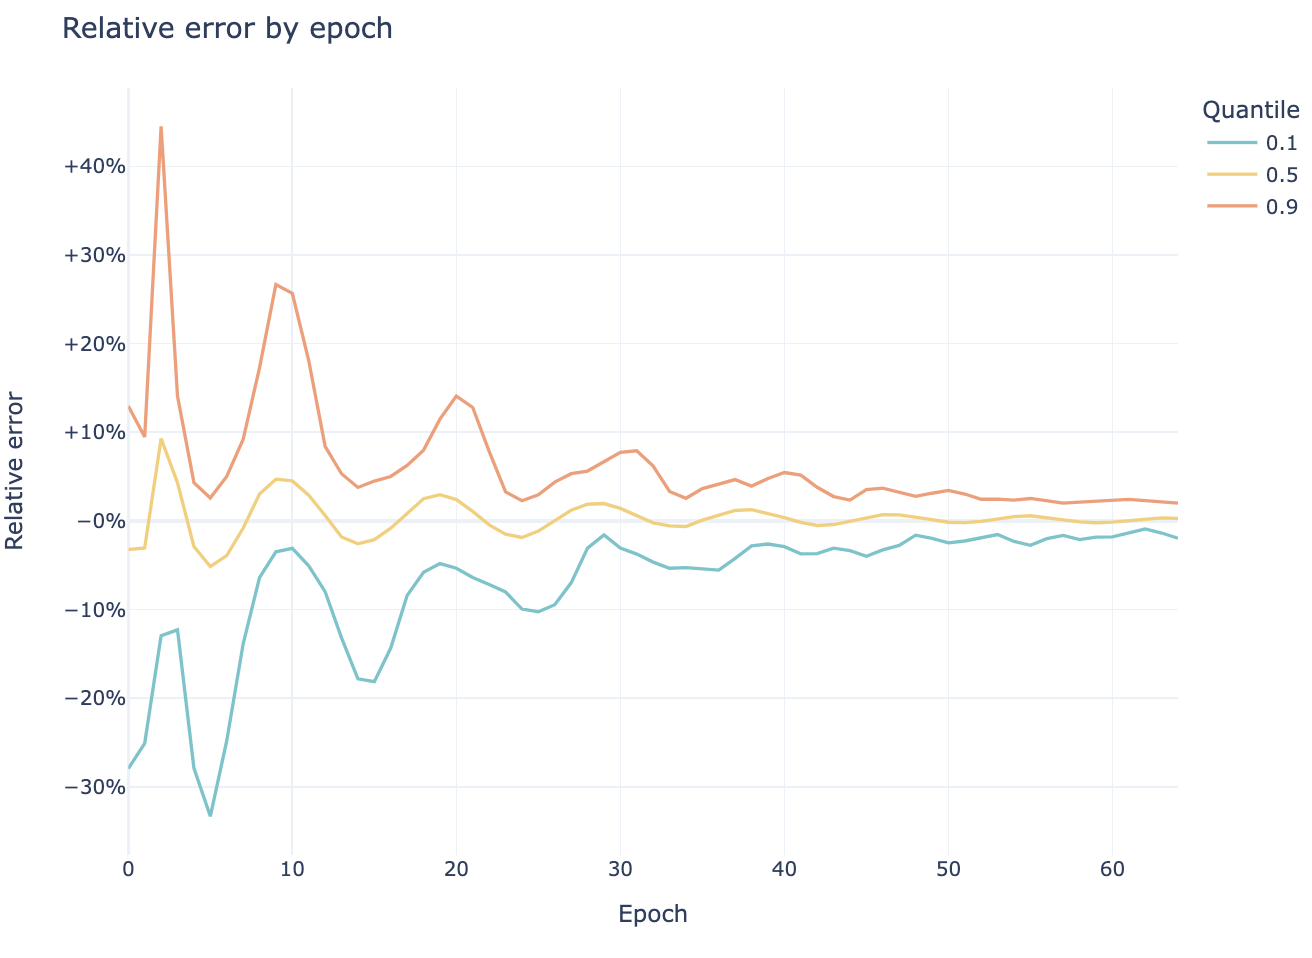
\includegraphics[width=0.45\textwidth]{rel_error_training.png}
  \caption{Distribution of relative error rates by epoch}
  \label{fig:rel_error_training}
\end{figure}

Fitting the entire set of statistical targets is challenging because it includes targets that are in conflict with each other, as well as in harmony. For example, employment income and Income Tax aggregates are correlated (and therefore if the survey moving further towards accurately reproducing one likely moves towards the other as well), but high-income-specific Income Tax aggregates are in conflict with the population of London (if the algorithm tries to hit the high-income-specific Income Tax aggregate by increasing the weights of high-income taxpayers, who are usually resident in London, it might quickly find that it has severely overestimated the regional population). This is a possible explanation for which the error rates in Figure \ref{fig:rel_error_training} are wave-like: the algorithm is in a constant state of trying to hit one target, but then finding that it has hit another target instead, and then trying to hit the first target again, and so on.

\subsection{Reform analysis comparison}

Baseline-only inference (how well a microsimulation model can describe the current household sector) is important, but the primary purpose of microsimulation models is to estimate the impact of a hypothetical \emph{reform} to policy rules. In order to validate not just the accuracy of the survey improvement method on the current baseline, but in reforms, we can measure how the optimised FRS compares to a source of `truth' for reform impacts. For example, the Dividend Allowance is a tax relief that exempts the first £2,000 of dividend income from Income Tax. Table \ref{tab:reform_comparison} compares microsimulation findings for the net cost of the tax relief\footnote{Defined as the difference in tax revenues compared to a scenario where it did not exist.} using the the original and enhanced FRS datasets against the estimates against HM Treasury's internal modelling (which uses the Survey of Personal Incomes, HMRC's administrative dataset).

\begin{table}[!ht]
  \caption{Comparison of reform impact estimates}
  \label{tab:reform_comparison}
  \centering
  \begin{tabular}{cc}
    \hline\hline
    Source & Estimate \\
    \hline
    HM Treasury (internal) & £720m \\
    Original FRS & £411m \\
    Enhanced FRS & £680m \\
  \hline\hline
  \end{tabular}
\end{table}

While there is no definite `source of truth' for hypothetical reforms, the SPI dataset is as close as we can get. This indicates the strength of the enhanced FRS dataset: suggesting that on this reform, it has combined the budgetary accuracy of the SPI (which is incapable of household microsimulation) with the applicability of the FRS.

\section{Evaluation}

Measuring the resultant accuracy against the actual data and models used by the established research groups inside and outside government is largely impossible, because all but one of the groups who carry out research using microsimulation do not publish standard model outputs or any validation against external statistics (this includes modelling groups inside and outside government)\footnote{The microsimulation models of note which cannot be used for comparison due to this are: the IFS' TAXBEN, `the IPPR model' at PERU, Manchester Metropolitan University, the DWP's PSM, HMRC's IGOTM.}. Only one model publishes validation statistics: UKMOD, managed by ISER at the University of Essex.

UKMOD publishes a comprehensive set of statistics regularly, detailing how the model's tax-benefit aggregate statistics compare to external aggregates.\cite{ukmod_country_report} A comparison of these results against the equivalent outputs from PolicyEngine-UK with the data enhancement methodology in this project shows the optimised FRS in this project outperforming UKMOD. Most aggregates in UKMOD's validation set have a relative error in the region of 10 to 30 percent against administrative truth; compared to 0 to 5 percent under the optimised datasets here.

\subsection{Non-negativity constraints on weights}

The optimisation process is constrained to non-negative weights, which is a reasonable assumption for a survey. However, experimentation with the optimisation process shows, as expected, that the optimiser can achieve a lower survey loss with this constraint removed. This raises an interesting and unorthodox question: do negative weights have a meaningful interpretation in the context of a survey? We might conclude that the intuitive meaning of the survey weight is not that a household record represents a negative number of households (which does not seem reasonable), but instead that the optimiser is trying to exploit the negativity to \emph{construct a new household record}: from the linear combination of the negative-weight household and some other positive-weighted household in the survey. Without the ability to alter individual household records, reweighting is the only way it can achieve this. Future research exploring this idea, as well as testing if this explanation can be intuitively demonstrated in the data (e.g. does this manifest as a simple household acting as a 'missing half', or is the actual function less intuitive?) could substantially increase the performance of the optimised weights and the survey as a whole.

\subsection{Other synthetic data generation methods}

Other methods exist for generating synthetic data. For example generative adversarial networks (GANs) have been shown to be highly effective at capturing and reproducing patterns arising from complex compositions of low-level data features. However, this approach (in this case, using conditional GANs) would likely have been less effective, for two reasons. Primarily, random forest models are inherently more robust to particular distributional features such as `bunching' (recall the capital gains example: tax policies often cause spikes at exact values of income amounts). Neural networks might approximate this, but with less precision than a decision tree. Secondly, modifiability: the random forest model architecture enables the distribution parameter adjustment `trick', but no such ability exists for GANs without significant modification, or retraining (which is costly).

Explainability is also key for microsimulation modelling. Given that outputs from the model are the result of aggregating tens of thousands of individual household outcomes, being able to interrogate characteristics of individual household records, \emph{and understand why they are a given value}, is essential for the model's results (which can often be counterintuitive) to retain legitimacy. With the random forest model distribution output, it is relatively straightforward to evaluate particular synthetics households. Figure \ref{fig:rf_interrogation} shows an interactive application developed for this purpose in this project, which allows the user to select input values for a given household, and simulate the random forest model's distribution outputs for the relevant income variables (reflecting the SPI income imputation stage of the enhancement process).

\begin{figure}[!ht]
  \centering
  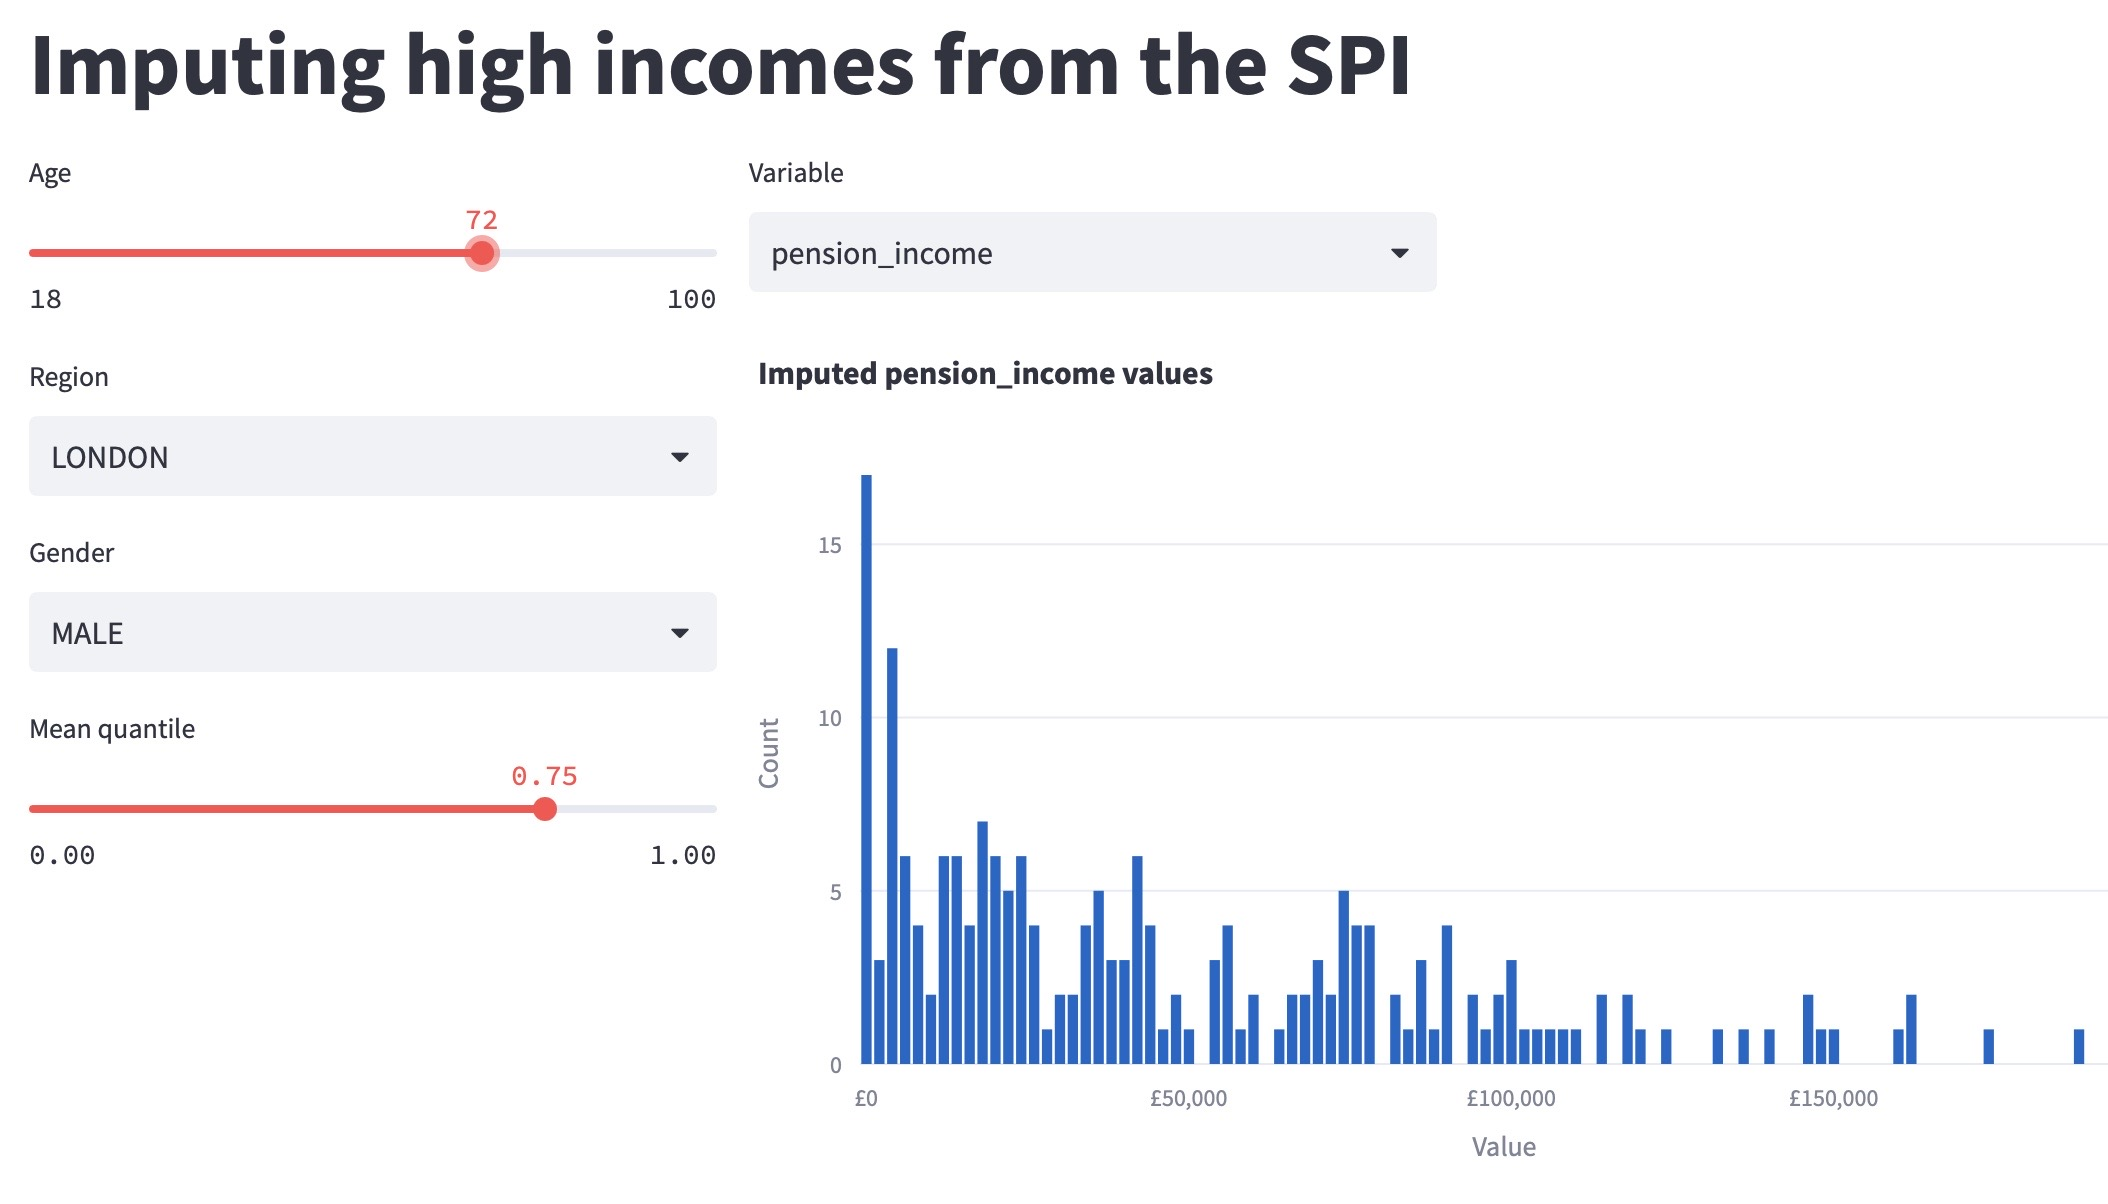
\includegraphics[width=0.45\textwidth]{rf_interrogation.jpeg}
  \caption{The synthetic data explorer}
  \label{fig:rf_interrogation}
\end{figure}


\subsection{Overfitting to statistical targets}

When directly targeting a set of statistical targets, there is a risk of overfitting to just those targets. For example, if we only fit the weights to tax statistics without also targeting demographic totals, we might find that the household population is significantly overestimated. This specific issue is solved by adding demographic targets to the loss function, but there will always be out-of-sample statistical targets: cross-tabulations by ethnicity, regional program statistics, etc. To test the severity of this issue, we can exclude a random percentage of the targets from the training loss function, and test how performance on those targets differs from the training targets. Cross-validation can also increase the robustness of this analysis, by rotating the selection used for validation to ensure no individual sample is under-represented in the validation set. Table \ref{tab:cross_validation} shows the results of this analysis, using 5-fold cross-validation.

\begin{table}[!ht]
  \caption{Cross-validation results}
  \label{tab:cross_validation}
  \centering
  \begin{tabular}{cc}
    \hline\hline
    Target & Final loss relative to original FRS \\
    \hline
    Training targets & -85\% \\
    Validation targets & -42\% \\
    Combined targets & -76\% \\
  \hline\hline
  \end{tabular}
\end{table}

This is also significantly better performance than the original FRS, which overfits to demographic targets \emph{by design}: FRS weights being optimised to hit population totals alone causes them to underfit financial targets in the way that they do.

One finding when carrying out this research was of the importance of not segmenting co-dependent targets between training and validation. For example, it was found that if the population targets for all regions except one (e.g. the South West) were in the training set and the remaining one was in the validation set, then the model was able to effectively exploit this by treating the population of the South West as a `spare household region' whose population did not matter and whose inhabitants could be used to plug any gaps in other targets as required.

\section{Conclusion}

The methods outlined in this project are independent of country profile or policy, requiring only a survey of reasonable accuracy and a set of target statistics of higher accuracy than the survey. The evaluation focussed on the UK, but the very same approaches could be applied to e.g. the United States or other jurisdictions, which often suffer from similar issues around under-reporting and sampling bias.

\subsection{Future research}

While the code to reproduce this enhanced FRS is publicly available, the actual dataset is limited to UK academic researchers and nonprofit organisations due to UK data licensing conditions. This limits the value that it can provide, increasing barriers to entry for potential new research and application. Countries like the United States do not impose this limitation (for example, the Current Population Survey, an analogue to the UK's FRS, is publicly available). This project used synthetic data techniques to \emph{extend}, rather than generate from scratch: future research investigating the possibility to create a new, calibrated FRS dataset with all the properties of the enhanced FRS would be a highly valuable contribution to the field, by enabling the resultant dataset to be made completely public.

Generating synthetic household data for this project is a complex task, primarily due to the fact that the FRS is a relational dataset: households can have variable numbers of members, and members have unique relationships with each other. Graph neural networks might be a promising approach to this problem, as they are able to model complex relationships between data points. However, the current state of the art in this area has not yet reached the same level of maturity as more established methods like regular ANNs, GANs, or random forests as in this implementation.



\subsection{Impact}

The positive results achieved in the UK context suggest a strong improvement in the accuracy of the FRS, and by extension the microsimulation model that uses the data. By combining the `best of both worlds` in granularity (from the FRS) and accuracy (from the SPI and other data sources), the pipeline effectively enables much more accurate (and consistent) microsimulation modelling of the UK tax-benefit system. Improving the accuracy of microsimulation modelling brings potentially sizeable improvements in the abilities of policymakers to understand the likely impacts of reforms to tax-benefit policy, and ultimately improve the effectiveness of such reforms in achieving their stated aims.

This project benefited from discussions and presentations made to other industry stakeholders across government, nonprofit and for-profit sectors. In particular, I presented the methodology and its applications to the HM Treasury internal distributional analysis team, who provided highly useful feedback and shed light on possible future applications. Other organisations and individuals also provided useful feedback and ideas for applications outside the scope of this project: for example, how using higher quality microdata for the random forest model imputations might affect the resultant optimised survey data quality.

\section*{Acknowledgements}

I would like to thank: my supervisor at the University of Durham, Professor Iain Stewart, for his guidance and support throughout this project; the many individuals and organisations who provided feedback and thoughts on the methodology and ideas behind it, including the HM Treasury distributional analysis team; the Joseph Rowntree Foundation modelling team; Matteo Richiardi at ISER and the IPPR model maintainers, as well as Max Ghenis at PolicyEngine for his extensive feedback on the project.

% trigger a \newpage just before the given reference
% number - used to balance the columns on the last page
% adjust value as needed - may need to be readjusted if
% the document is modified later
%\IEEEtriggeratref{8}
% The "triggered" command can be changed if desired:
%\IEEEtriggercmd{\enlargethispage{-5in}}

% references section

% can use a bibliography generated by BibTeX as a .bbl file
% BibTeX documentation can be easily obtained at:
% http://mirror.ctan.org/biblio/bibtex/contrib/doc/
% The IEEEtran BibTeX style support page is at:
% http://www.michaelshell.org/tex/ieeetran/bibtex/
%\bibliographystyle{IEEEtran}
% argument is your BibTeX string definitions and bibliography database(s)
%\bibliography{IEEEabrv,../bib/paper}
%
% <OR> manually copy in the result`ant .bbl file
% set second argument of \begin to the number of references
% (used to reserve space for the reference number labels box)

\newpage

\bibliography{IEEEabrv,../references}
% Use the APA style bibliography (requires natbib)
\bibliographystyle{apalike}

% that's all folks
\end{document}


